\documentclass[11pt]{article}       % The percent symbol in your code starts a comment.  The comment ends at the next linebreak.
\usepackage[english]{babel}         % Packages add functionality and style conventions to your documents. Don't edit this section!
\usepackage{fullpage}               % Eliminates wasted space
\usepackage[utf8]{inputenc}         % Necessary for character encoding
\usepackage{amsmath, amssymb,amsthm}% Required math packages
\usepackage{graphicx}               % For handling graphics
\usepackage[colorinlistoftodos]{todonotes}  % For the fancy "todo" stuff
\usepackage{hyperref}               % For clickable links in the final PDF
\usepackage{tikz}
\theoremstyle{definition}
\newtheorem{theorem}{Theorem}
\newtheorem{lemma}[theorem]{Lemma}
\newtheorem{prop}[theorem]{Proposition}
\newtheorem{claim}[theorem]{Claim}

\title{Complex Analysis -- Homework \#16}

\author{Josenjamonnor Komissalluman}

\date{ Due Wednesday, March 17, 2021 }

\begin{document}
\color{white}
\pagecolor{black}

\maketitle

\noindent{\bf 1. }   This problem is a throw-back to, and extension of, problem 1 of Homework \#5 in which we essentially proved that if $|\alpha| < 1$, then the fractional linear transformation $w=f(z)=\dfrac{z-\alpha}{1-\overline{\alpha}z}$ is a conformal mapping of the unit disk onto itself.
\vskip.05in

\noindent{\bf a. }  Prove that if distinct \emph{real} numbers $a$ and $b$ in the interior of the unit disk are mapped to  \emph{real}  numbers $f(a)$ and $f(b)$, then $\alpha \in \mathbb R$.

Observe that
\begin{align*}
         f(a) &= \frac{a-\alpha}{1 - \overline\alpha a}, \\
\implies a-\alpha &= f(a) - f(a)\overline\alpha a, \\
\implies \alpha &= a - f(a) + f(a)\overline\alpha a.
\end{align*}
Then,
\begin{align*}
         f(b) &= \frac{b-\alpha}{1-\overline\alpha b} \\
              &= \frac{b - (a - f(a) + f(a)\overline\alpha a)}{1-\overline\alpha b} \\
              &= \frac{b-a+f(a)-f(a)\overline\alpha a}{1-\overline\alpha b}, \\
\implies f(b) - f(b)\overline\alpha b &= b-a+f(a)-f(a)\overline\alpha a, \\
\implies f(a)\overline\alpha a - f(b)\overline\alpha b &= b-a+f(a) - f(b), \\
\implies \overline\alpha(f(a)a - f(b)b) &= b-a+f(a) - f(b), \\
\implies \overline\alpha &= \frac{b-a+f(a) - f(b)}{f(a)a - f(b)b}.
\end{align*}
Thus, $\overline\alpha$ is a real number, so $\alpha$ is a real number.

\newpage
\noindent
\dotfill

\noindent{\bf b. }  Map the region bounded by the circles $|z|=1$ and $|z-\frac14|=\frac14$ conformally onto an annulus  $\rho < |w| < 1$.
\vskip.1in
\centerline{
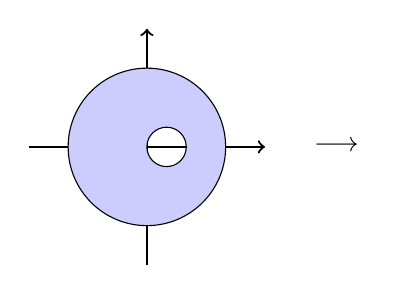
\begin{tikzpicture}
\draw[thick,->] (-1.5,0) -- (1.5,0);
\node [right ] at (2,0) {$\longrightarrow$};
\draw[thick,->] (0,-1.5) -- (0,1.5);
  \fill[blue!20,even odd rule] (1/4,0) circle (1/4) (0,0) circle (1);
    \draw (1/4,0) circle (0.25cm);
\draw (0,0) circle (1cm);
\end{tikzpicture}
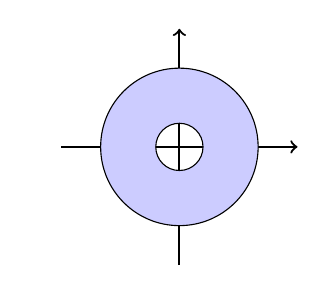
\begin{tikzpicture}
\draw[thick,->] (-1.5,0) -- (1.5,0);
\draw[thick,->] (0,-1.5) -- (0,1.5);
\node [left ] at (-1.5,0) {\phantom{x}};
  \fill[blue!20,even odd rule] (0,0) circle (0.3) (0,0) circle (1);
  \draw (0,0) circle (0.3cm);
\draw (0,0) circle (1cm);
\end{tikzpicture}
}


\vskip.1in
\hrule


\end{document}